\documentclass[11pt]{article}

\usepackage[margin=1in]{geometry}
\usepackage[T1]{fontenc}
\usepackage{array}
\usepackage{tikz}
\usetikzlibrary{arrows.meta,positioning}

\title{FSM Interpretation for min-mayus-letter-FPGA}
\author{}
\date{\today}

\begin{document}

\maketitle

\section*{Project Context}

The current \texttt{VERIFICATION/min-mayus-letter-FPGA/src/top.v} file only
instantiates \texttt{uart\_rx} and \texttt{uart\_tx}. The whiteboard process is
therefore interpreted as a small supervisory finite-state machine placed above
those two UART blocks.

\begin{center}
\begin{tabular}{|>{\ttfamily}p{0.28\linewidth}|>{\ttfamily}p{0.28\linewidth}|p{0.28\linewidth}|}
\hline
Whiteboard signal & Project signal & Meaning \\
\hline
Rx.done & rx\_done & One-cycle pulse when a byte has been received \\
\hline
Rx.rx\_data & rx\_data & Received byte from \texttt{uart\_rx} \\
\hline
Tx.tx\_data & tx\_data & Byte presented to \texttt{uart\_tx} \\
\hline
Tx.tx\_start & tx\_en & Request to start transmission \\
\hline
Tx.busy & tx\_busy & Transmitter is currently sending a frame \\
\hline
\end{tabular}
\end{center}

\section*{Behavior Extracted from the Image}

\begin{enumerate}
    \item Wait until \texttt{rx\_done = 1}.
    \item If \texttt{rx\_data} is an ASCII lowercase letter
    (\texttt{97 <= rx\_data <= 122}), convert it to uppercase by subtracting
    \texttt{32}.
    \item Otherwise, keep the byte unchanged.
    \item Wait until the transmitter is idle (\texttt{tx\_busy = 0}).
    \item Assert \texttt{tx\_en}.
    \item Keep \texttt{tx\_en} asserted until \texttt{tx\_busy} goes high,
    which acknowledges that the UART transmitter accepted the byte.
    \item Deassert \texttt{tx\_en} and return to the receive-wait state.
\end{enumerate}

\section*{Proposed Supervisory FSM}

\begin{center}
\resizebox{\linewidth}{!}{%
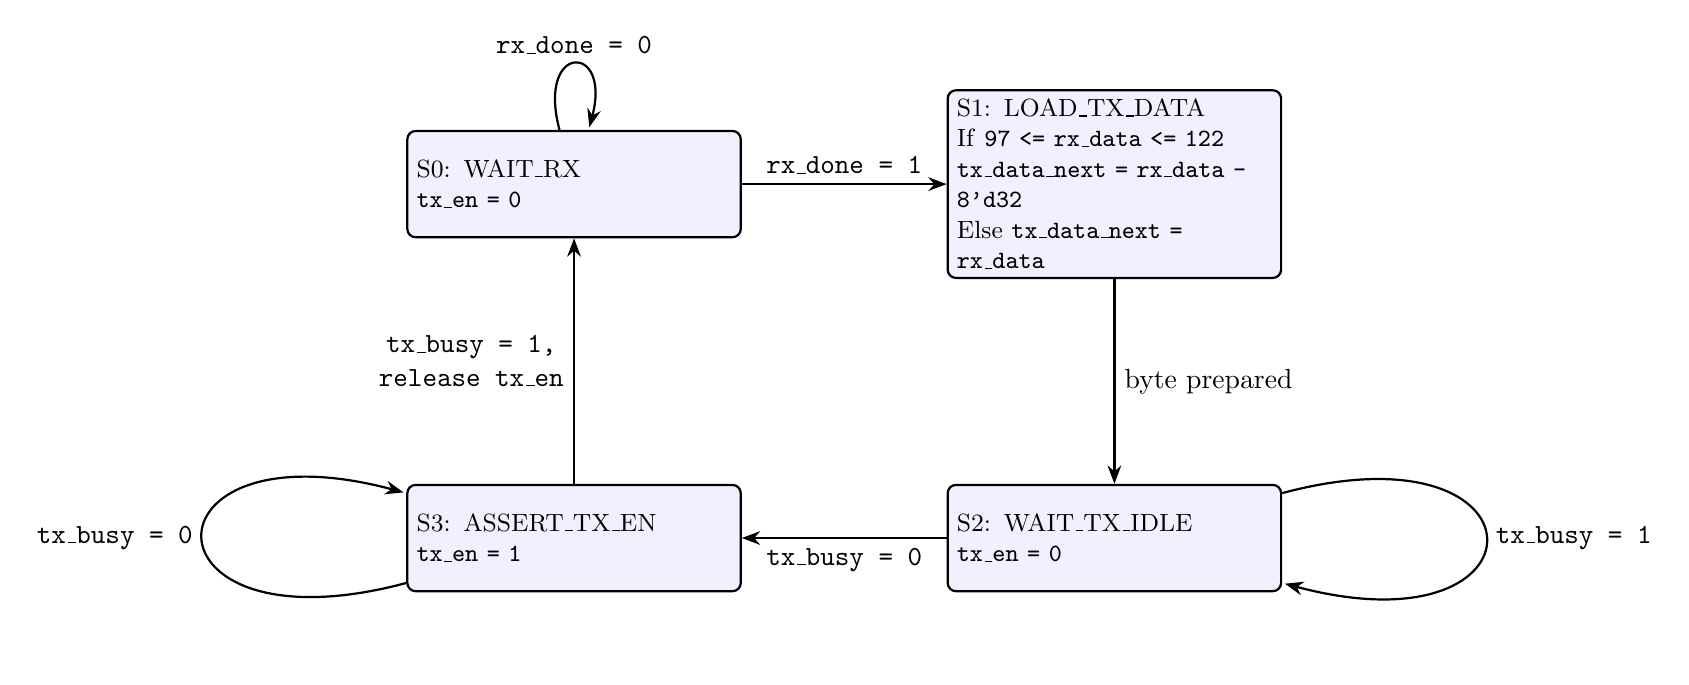
\begin{tikzpicture}[
    >=Stealth,
    node distance=2.6cm and 2.6cm,
    statebox/.style={
        draw,
        rounded corners=3pt,
        thick,
        align=left,
        text width=4.0cm,
        minimum height=1.35cm,
        fill=blue!6,
        font=\small
    },
    line/.style={->, thick}
]
    \node[statebox] (waitrx) {S0: WAIT\_RX\\\texttt{tx\_en = 0}};
    \node[statebox, right=of waitrx] (loadtx) {S1: LOAD\_TX\_DATA\\If \texttt{97 <= rx\_data <= 122}\\\texttt{tx\_data\_next = rx\_data - 8'd32}\\Else \texttt{tx\_data\_next = rx\_data}};
    \node[statebox, below=of loadtx] (waitidle) {S2: WAIT\_TX\_IDLE\\\texttt{tx\_en = 0}};
    \node[statebox, left=of waitidle] (starttx) {S3: ASSERT\_TX\_EN\\\texttt{tx\_en = 1}};

    \draw[line] (waitrx) edge[loop above] node {\texttt{rx\_done = 0}} (waitrx);
    \draw[line] (waitrx) -- node[above] {\texttt{rx\_done = 1}} (loadtx);
    \draw[line] (loadtx) -- node[right] {byte prepared} (waitidle);
    \draw[line] (waitidle) edge[loop right] node {\texttt{tx\_busy = 1}} (waitidle);
    \draw[line] (waitidle) -- node[below] {\texttt{tx\_busy = 0}} (starttx);
    \draw[line] (starttx) edge[loop left] node {\texttt{tx\_busy = 0}} (starttx);
    \draw[line] (starttx) -- node[left, align=center] {\texttt{tx\_busy = 1,}\\\texttt{release tx\_en}} (waitrx);
\end{tikzpicture}
}
\end{center}

\section*{State Notes}

\begin{itemize}
    \item \textbf{S0: WAIT\_RX} corresponds to step 1 in the whiteboard text.
    \item \textbf{S1: LOAD\_TX\_DATA} implements step 1.1 and decides whether
    the received byte must be converted from lowercase to uppercase.
    \item \textbf{S2: WAIT\_TX\_IDLE} matches step 1.2 and prevents a new send
    request while the transmitter is still busy.
    \item \textbf{S3: ASSERT\_TX\_EN} matches step 1.3. The state holds the
    start request until the TX block acknowledges it by raising
    \texttt{tx\_busy}.
\end{itemize}

\section*{Implementation Remark}

This FSM is not yet present in the current project top-level. The existing
\texttt{top.v} exposes the UART interfaces, but a controller register for
\texttt{tx\_data} plus an FSM for \texttt{tx\_en} would still need to be added
if the whiteboard behavior is to become synthesizable RTL.

\end{document}
